\documentclass[letterpaper, 12pt]{article}

\usepackage[utf8]{inputenc}
\usepackage[english, spanish]{babel}
\usepackage{fullpage}
\usepackage{graphicx}
\usepackage{amsmath}
\usepackage{enumitem}
\usepackage{chngcntr}
\usepackage{setspace}
\usepackage{url}
\usepackage{csquotes}
\usepackage{float}
\usepackage{verbatim}
\usepackage{tabularx}
\usepackage{amsmath}
\usepackage{caption}
\usepackage{bm}
% \usepackage{hyperref}

\counterwithin{figure}{section}
\renewcommand{\thesection}{\arabic{section}}
\renewcommand{\thesubsection}{\thesection.\arabic{subsection}}
\renewcommand{\baselinestretch}{1.5}
\renewcommand{\thefigure}{\arabic{figure}}

\usepackage[style=numeric, maxnames=6, minnames=3, backend=biber, parentracker=true, sorting=none]{biblatex}
\DefineBibliographyStrings{english}{%chktex-file 1 chktex-file 6
	andothers = {\em et\addabbrvspace al\adddot}
}
\addbibresource{./Bibliography/bibliography.bib}

\usepackage{array}
\usepackage{enumitem}

\setlength{\parskip}{20pt}

\newcommand{\bolditalic}[1]{\textbf{\textit{#1}}}

% chktex-file 24

\begin{document}

\begin{titlepage}
	\centering
	
\includegraphics[width=0.3\textwidth]{Images/logo_utb.png}\par\vspace{1cm}
	{\scshape\LARGE Universidad Tecnológica de Bolívar \par}
	\vspace{1cm}

	{\scshape\Large FÍSICA CALOR Y ONDAS \par}
	\vspace{2.5cm}

	% chktex-file 8
	\slshape {\Large \bfseries{} Avance del proyecto No. II \\}
	\vspace{2cm}

	\slshape {\itshape{} Mauro González, T00067622 \\}
	\slshape {\itshape{} German De Armas Castaño, T00068765 \\}
	\slshape {\itshape{} Angel Vega Rodriguez, T00068186 \\}
	\slshape {\itshape{} Juan Jose Osorio Ariza, T00067316 \\}
	\slshape {\itshape{} Jorge Rueda Salgado, T00068722 \\}
	\vfill
	Revisado Por \\
	Yady Tatiana Solano Correa\\
	{\large \today\par}
\end{titlepage}

% ! --------------------------------------------------------------------------------------------------------------------------------|>
\section*{\textit{Resumen}}

\begin{quote}
	En el vasto universo de la física, pocas cosas son tan omnipresentes
	como las ondas. En el caso de nuestro proyecto, nos enfocamos en
	la lectura de ondas sonoras y su presencia en el mundo cotidiano.
	Para este segundo informe de avance, mostraremos los logros alcanzados
	hasta el momento, plasmando nuestra idea primigenia del proyecto en un
	programa básico. En este programa, se recopilan estas ondas
	sonoras (ya sea a través de canciones, grabaciones, etc.) para
	luego enviarlas a un servidor y ser representadas mediante
	gráficas, mostrando sus propiedades básicas.

	Hemos implementado un tipo de filtro que nos permite
	mostrar únicamente la información que es de nuestro
	interés, desentrañando sus características y propiedades
	fundamentales, tales como el espectro de la onda, el tempo,
	el ritmo y sus coeficientes centrales en las frecuencias
	Mel (MFCC). Todo esto con la idea de que sea aplicable en
	diversos campos, como la música, la medicina o la ciencia
	de datos.
\end{quote}

% ! --------------------------------------------------------------------------------------------------------------------------------|>

\noindent\makebox[\linewidth]{\rule{\linewidth}{0.4pt}}

\bolditalic{Palabras claves}: \textit{Ondas sonoras, ondas electromiográficas,
	ingeniería del sonido, síntesis de sonido, espectro de
	onda.}

\noindent\makebox[\linewidth]{\rule{\linewidth}{0.4pt}}

% ! --------------------------------------------------------------------------------------------------------------------------------|>
\section*{Objetivos}

% + -------------------------------------------------------------------------|>
\subsection*{Objetivo general}

Diseñar una herramienta de lectura de ondas con el
propósito de adquirir, analizar y visualizar los datos
generados por ondas provenientes de distintas fuentes o
fenómenos, contribuyendo así a la comprensión y estudio de
sus características y patrones, que tenga el potencial de
evolucionar hacia una plataforma avanzada en el futuro.

% + -------------------------------------------------------------------------|>
\subsection*{Objetivos específicos}

\begin{itemize}[label=$\triangleright$]
	\item Realizar varias pruebas para garantizar que el programa
	      funcione de manera óptima y sea capaz de manejar una
	      variedad de formatos de audio.

	\item Representar gráficamente las propiedades fundamentales de
	      una onda sonora y su espectrograma.
\end{itemize}

% ! --------------------------------------------------------------------------------------------------------------------------------|>
\section*{Marco Teorico}

% + -------------------------------------------------------------------------|>
\subsection*{Ondas~\cite{onda_concepto}}

Se conoce como onda a la propagación de energía (y no de
masa) en el espacio debido a la perturbación de alguna de
sus propiedades físicas, como son la densidad, presión,
campo eléctrico o campo magnético. Este fenómeno puede
darse en un espacio vacío o en uno que contenga materia, ya
sea agua, aire, tierra, etc.

% + -------------------------------------------------------------------------|>
\subsection*{Ondas sonoras~\cite{ondas_sonoras}}

Una onda sonora es una onda expansiva que puede ser
percibida por el oído humano. La onda sonora se puede
generar a partir del aparato fonador humano, mediante
máquinas, por animales, etc. Ademas se puede propagar en
distintos medios.

\begin{itemize}[label=$\triangleright$]
	\item Amplitud [A]: Es la magnitud máxima del desplazamiento con
	      respecto al equilibrio, es decir, es la distancia existente
	      entre la posición de equilibrio y cualquiera de las
	      posiciones extremas. Su unidad de medidas en el Sistema
	      Internacional es el metro \bolditalic{(m)}.

	      \begin{equation*}
		      A = \sqrt{X_{0}^{2} + \frac{V_{0x}^{2}}{\omega^{2}}}
	      \end{equation*}

	\item Periodo [T]: Es el tiempo que tarda una oscilación completa
	      (ciclo), y siempre es positivo. La unidad del periodo en el
	      SI es el segundo \bolditalic{}{(s)}, aunque a veces se
	      expresa como “segundos por ciclo”.

	\item Frecuencia [f]: Es el número de ciclos en la unidad de
	      tiempo, y siempre es positiva. La unidad de la frecuencia
	      en el SI es el Hertz (Hz).

	      1 Hz = 1 oscilación/segundo = $1s^{-1}$

\end{itemize}

% + -------------------------------------------------------------------------|>
\subsection*{Espectrómetro de sonido~\cite{espectometro}}

Es un dispositivo o programa informático que se utiliza
para visualizar y analizar las características espectrales
de una señal de audio. Básicamente, descompone una señal de
audio en sus componentes de frecuencia para proporcionar
información detallada sobre la distribución de energía en
diferentes bandas de frecuencia. Un espectrómetro de sonido
puede proporcionar información detallada sobre la amplitud
y frecuencia de los componentes de una señal de audio. Es
importante destacar que tanto hardware como software pueden
desempeñar el papel de un espectrómetro de sonido. En el
caso de software, librerías como ``libros'' en Python
pueden ser utilizadas para implementar funcionalidades de
espectro de sonido en aplicaciones de procesamiento de
audio.

% + -------------------------------------------------------------------------|>
\subsection*{Espectrograma~\cite{espectograma}}

Un espectrograma es una representación visual de cómo varía
la energía de una señal de audio en función del tiempo y la
frecuencia. La lectura o comprensión del espectrómetro es
la siguiente: Eje horizontal (eje del tiempo): Representa
el tiempo en el eje horizontal, generalmente de izquierda a
derecha. Cada punto en este eje corresponde a un momento
específico en la grabación de audio.

Eje vertical (eje de frecuencia): Las frecuencias más bajas
suelen estar en la parte inferior, mientras que las
frecuencias más altas están en la parte superior.

Intensidad del color o brillo: Indica la amplitud o energía
de cada frecuencia en un momento específico. Los colores
más oscuros o brillantes indican una mayor energía en esa
frecuencia en ese momento particular.

% + -------------------------------------------------------------------------|>
\subsection*{Intensidad de sonido~\cite{diapos}}

La intensidad de sonido se refiere a la cantidad de energía
que transporta una onda de sonido por unidad de área en una
dirección perpendicular al flujo de la onda. En términos
más simples, la intensidad de sonido representa cuán fuerte
o débil es una onda sonora en un punto específico del
espacio. La intensidad de sonido se mide en vatios por
metro cuadrado (W/m²) y puede variar ampliamente en
diferentes situaciones.

\begin{equation*}
	I = \frac{\frac{E}{t}}{A} = \frac{P}{A}
\end{equation*}

% + -------------------------------------------------------------------------|>
\subsection*{Decibeles~\cite{diapos}}

Son una unidad de medida que se utiliza para expresar la
relación entre dos cantidades, generalmente en términos de
potencia, intensidad o nivel de presión.

\begin{equation*}
	\beta = 10 \log{\frac{I}{I_{0}}}
\end{equation*}

Donde $I_{0}$ es $10^{-12}\frac{W}{m^{2}}$

% + -------------------------------------------------------------------------|>
\subsection*{MFCC~\cite{mfcc}}

Los Coeficientes Ceptrales en las Frecuencias de Mel (MFCC,
por sus siglas en inglés: Mel Frequency Cepstral
Coefficients) son una representación de las características
espectrales de una señal de audio, diseñada para imitar
ciertas características del sistema auditivo humano. El
proceso para obtener MFCC generalmente involucra los
siguientes pasos:

\begin{enumerate}
	\item División en tramas (frames): La señal de audio se divide en
	      pequeñas tramas, típicamente de 20 a 30 milisegundos de
	      duración. Cada trama se superpone ligeramente con la
	      siguiente para asegurar la continuidad de la información.

	\item Transformada de Fourier: Para cada trama, se aplica una
	      transformada de Fourier para convertir la señal del dominio
	      del tiempo al dominio de la frecuencia. Esto da como
	      resultado un espectrograma, que muestra cómo la energía
	      está distribuida en diferentes frecuencias en esa trama.

	\item Filtro de Frecuencias Mel: Se aplica un conjunto de filtros
	      de frecuencias Mel para el espectrograma. Los filtros de
	      frecuencias Mel están diseñados para imitar la respuesta
	      del oído humano, que no percibe las frecuencias de manera
	      lineal, sino de una forma más logarítmica. Esto significa
	      que somos más sensibles a las diferencias en frecuencias
	      bajas que en frecuencias altas.

	\item Aplicación del Logaritmo: Se toma el logaritmo de la
	      energía en cada uno de los filtros Mel. Esto hace que la
	      representación sea más parecida a cómo percibimos el
	      sonido.

	\item Transformada Cepstral Discreta (DCT): Finalmente, se aplica
	      una transformada cepstral discreta para obtener los
	      coeficientes ceptrales. Esta transformación se realiza para
	      reducir la redundancia en la representación de las
	      características y obtener un conjunto compacto de
	      características que sea eficaz para el reconocimiento del
	      habla y otras aplicaciones de procesamiento de audio.
\end{enumerate}

% + -------------------------------------------------------------------------|>
\subsection*{Tonalidad en el sonido~\cite{tonalidad}}

La tonalidad en el contexto del sonido se refiere a la
percepción subjetiva de la altura o agudeza de un tono
musical. En otras palabras, la tonalidad nos dice si un
sonido se percibe como agudo o grave. La tonalidad está
directamente relacionada con la frecuencia de una onda
sonora. Frecuencias más altas corresponden a tonos más
agudos, mientras que frecuencias más bajas corresponden a
tonos más graves. En el sistema musical occidental, la
tonalidad se organiza en una escala cromática compuesta por
12 tonos, cada uno separado por un semitono. Cada tono
tiene una frecuencia específica asociada y está etiquetado
con una nota musical (por ejemplo, Do, Re, Mi, etc.). La
repetición de estas 12 notas a lo largo del teclado de un
piano, por ejemplo, constituye lo que se conoce como una
octava.

% ! --------------------------------------------------------------------------------------------------------------------------------|>
\section*{Procedimiento experimental}

\begin{enumerate}
	\item Inicio del programa
	\item Pedir al usuario que seleccione un archivo
	      \begin{figure}[H]
		      \begin{center}
			      
\includegraphics[width=.5\linewidth]{./Images/FileUploadColab.PNG}
			      \caption{}
		      \end{center}
	      \end{figure}

	      Debido a la naturaleza de la herramienta en la que se
	      desarrollo el programa, se abrirá un \textit{Botón} en el
	      que el usuario puede dar click para seleccionar un archivo.

	      \begin{figure}[H]
		      \begin{center}
			      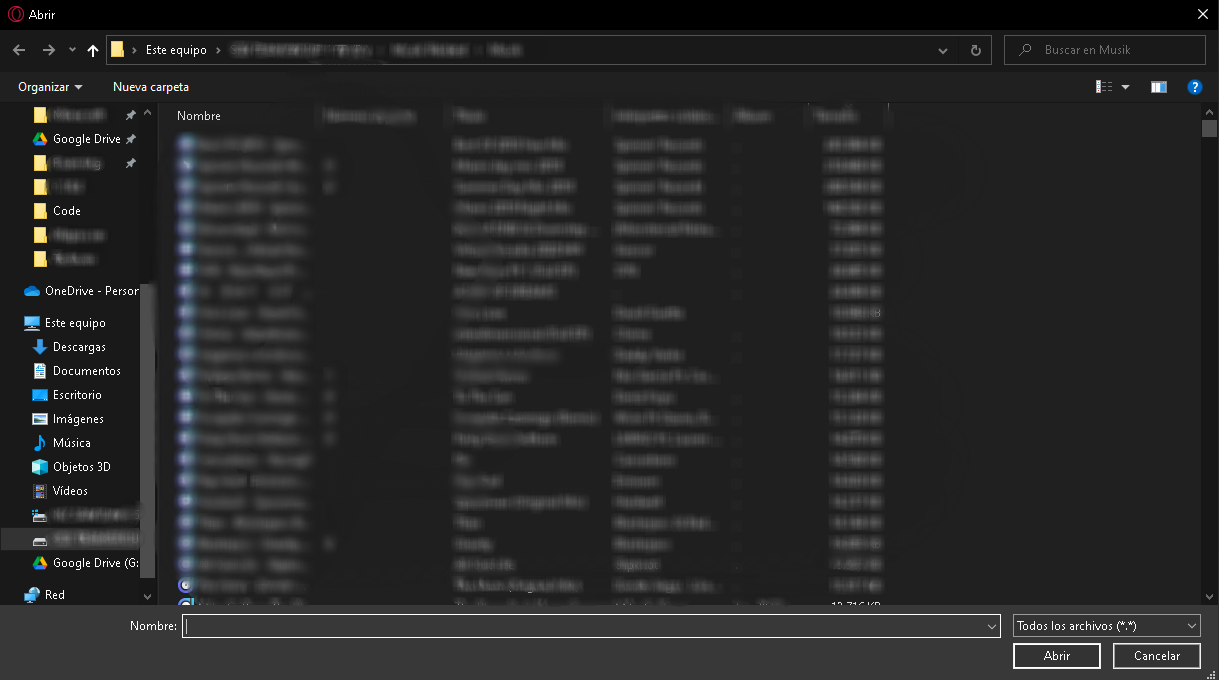
\includegraphics[width=.7\linewidth]{./Images/FileExplorer.png}
			      \caption{}
		      \end{center}
	      \end{figure}

	      Luego, se utiliza el explorador de archivos, para luego
	      proceder con la carga.

	\item Proceder con la carga del archivo a las librerías

	      \begin{figure}[H]
		      \begin{center}
			      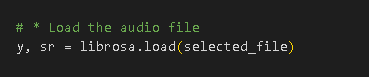
\includegraphics[width=.5\linewidth]{./Images/LoadFile.PNG}
			      \caption{}
		      \end{center}
	      \end{figure}

	      En caso de que el archivo contenga algún error, o
	      directamente no se pueda acceder a él, en ese caso el
	      programa lanzaría una \textit{Exception}, procediendo con
	      la terminación de la ejecución. Caso contrario, se procede
	      con el resto de la ejecución.

	\item Realizar el análisis de audio

	      Luego de verificar que no haya errores en el archivo de
	      audio, se procede a extraer las características que
	      consideremos pertinentes.

	      \begin{figure}
		      \begin{center}
			      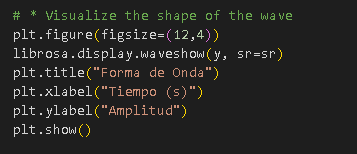
\includegraphics[width=.7\linewidth]{./Images/AudioAnalysisSample_1.PNG}
			      \caption{Bloque de muestra}
		      \end{center}
	      \end{figure}

	      La extracción de características consiste en pequeños
	      bloques, en los que cada uno de estos renderiza la
	      información para ser vista por el usuario.

	      \begin{figure}[H]
		      \begin{center}
			      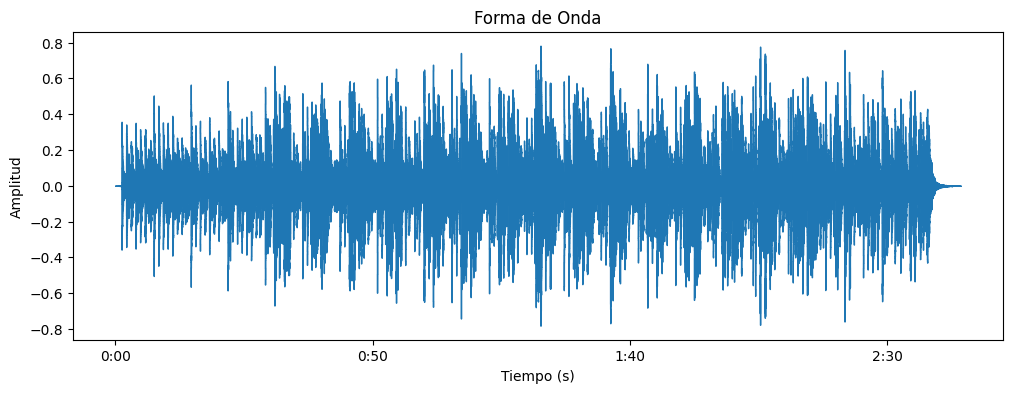
\includegraphics[width=.7\linewidth]{./Images/SampleRunImage_1.png}
			      \caption{}
			      \label{figure:sample_run_image_1}
		      \end{center}
	      \end{figure}

	      La anterior imagen~(\ref{figure:sample_run_image_1}), da un
	      pequeño ejemplo de como seria el \textit{Output final} del
	      programa.
\end{enumerate}

Todo esto se vería resumido en el siguiente flujograma:

\begin{figure}[H]
	\begin{center}
		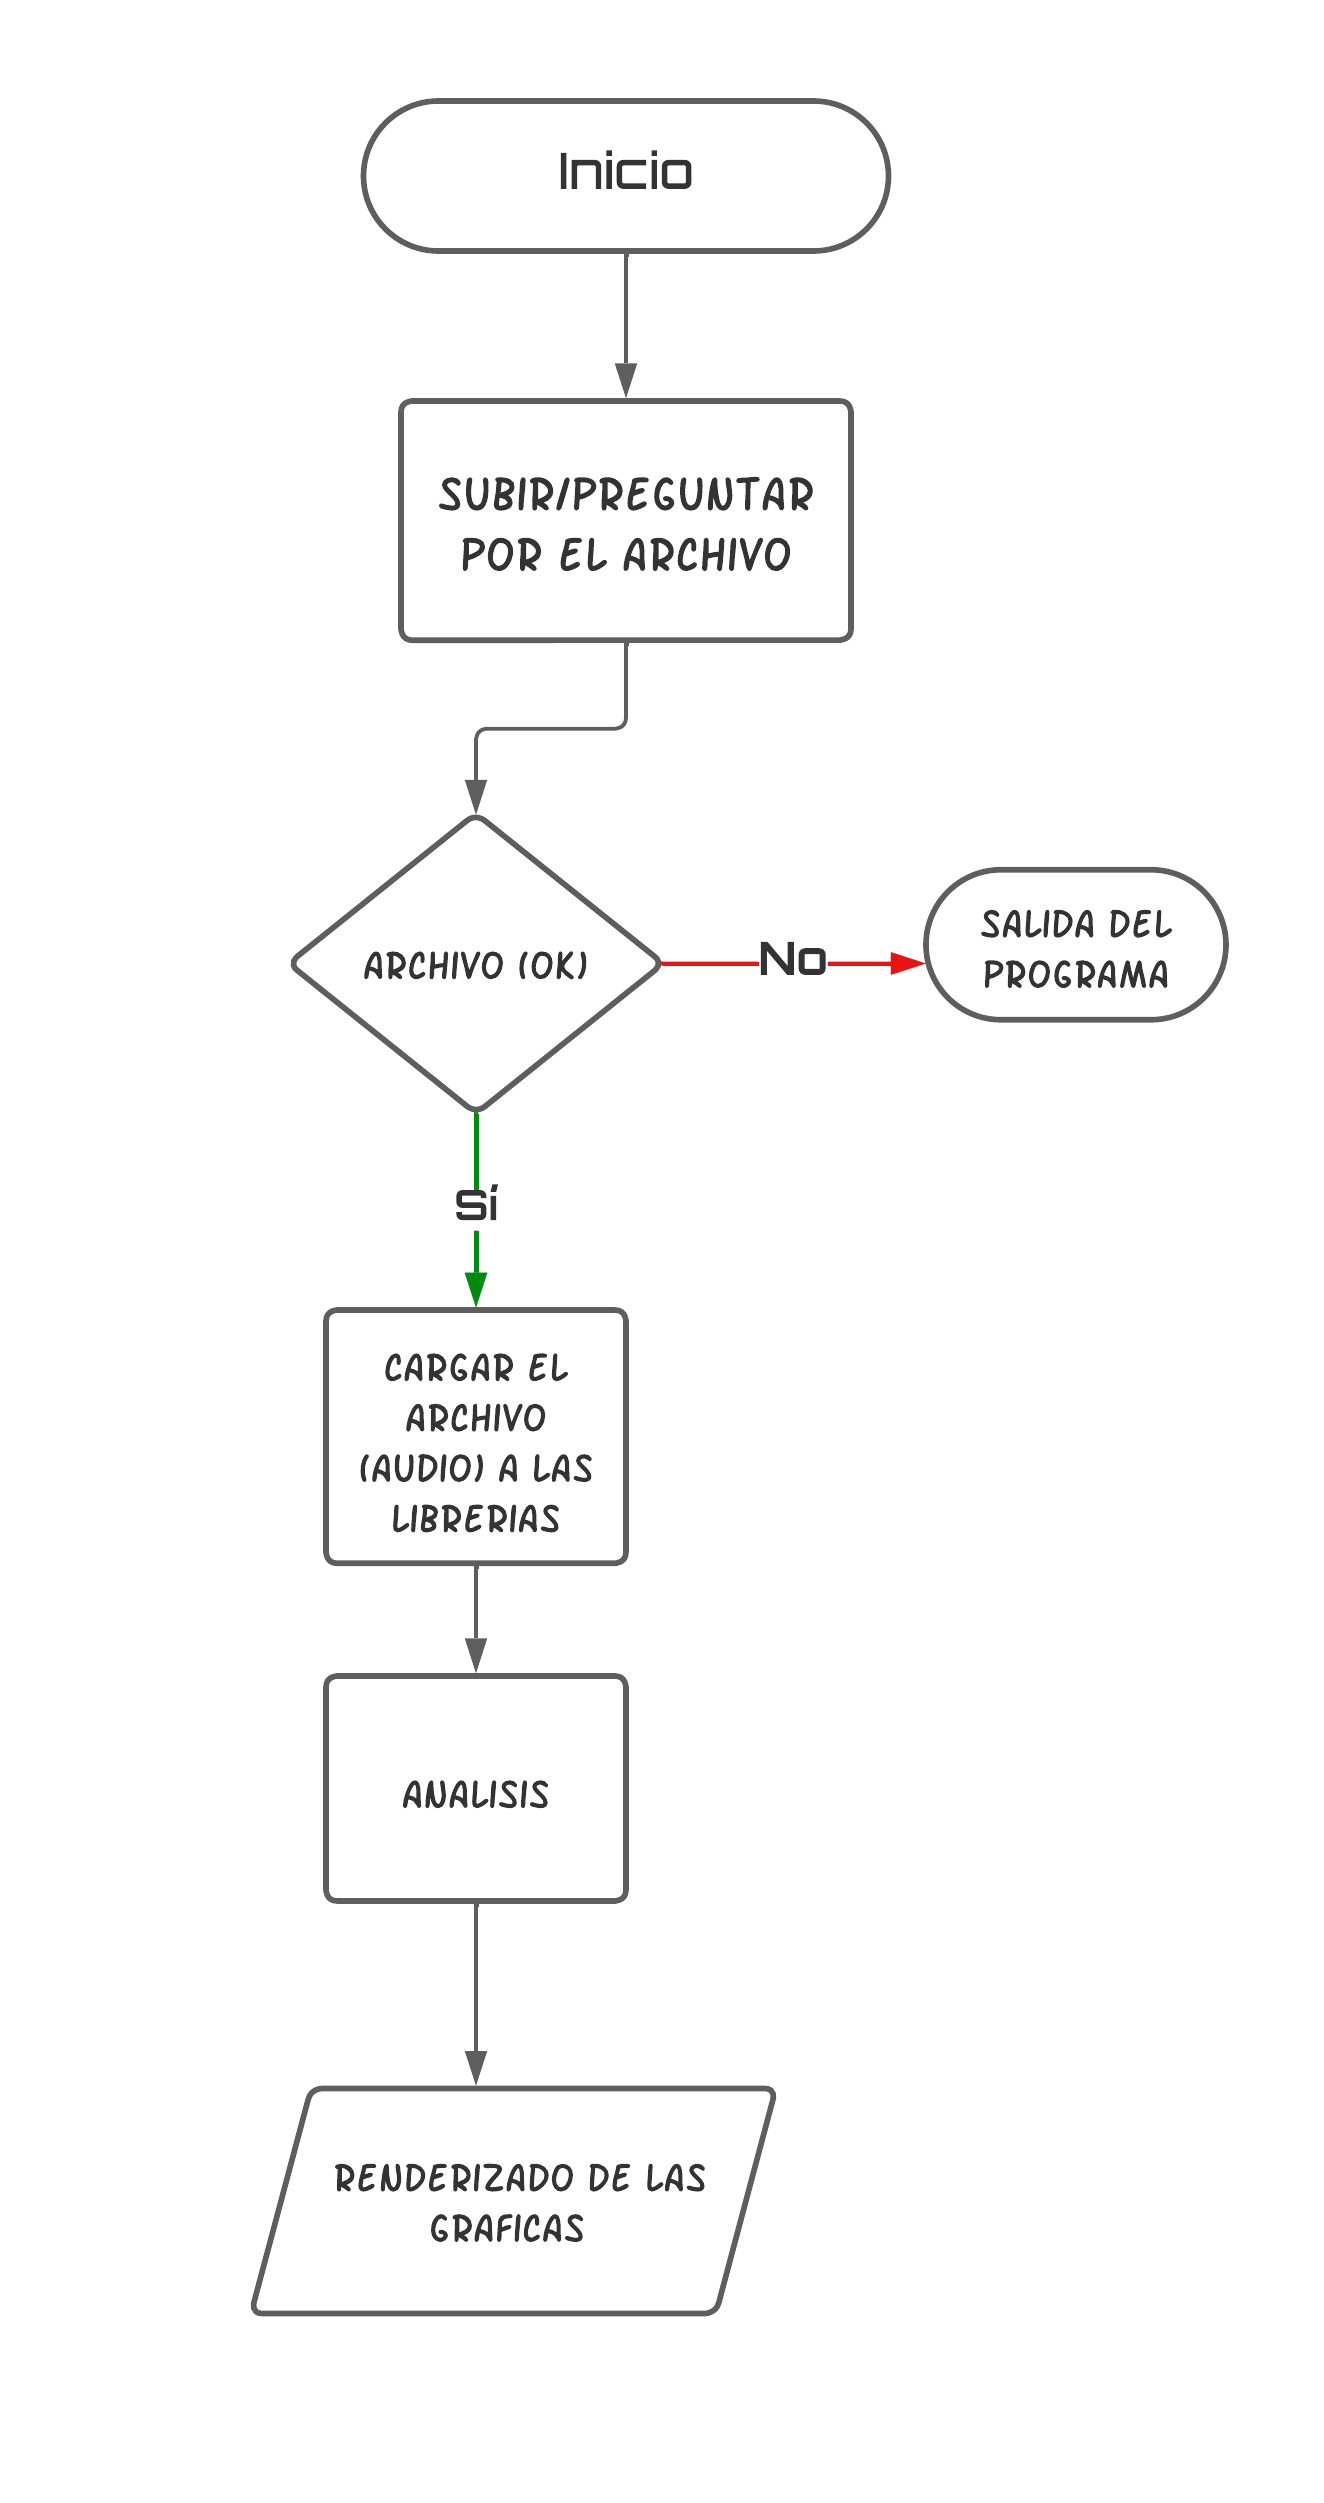
\includegraphics[width=.6\linewidth]{./Images/Flujograma.png}
		\caption{}
	\end{center}
\end{figure}

% ! --------------------------------------------------------------------------------------------------------------------------------|>
\section*{Datos experimentales}

Para evaluar el desempeño de nuestro programa, hemos
empleado la canción ``Rap God'' de \textit{Eminem}. A
continuación, presentaremos los resultados obtenidos.

\begin{figure}[H]
	\begin{center}
		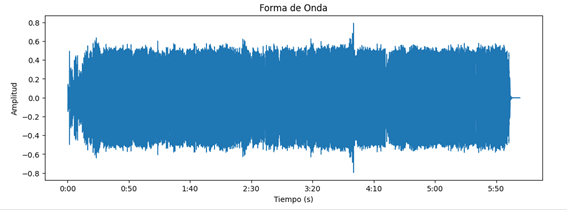
\includegraphics[width=.7\linewidth]{./Images/DatosExperimentales_1.png}
		\caption{}
	\end{center}
\end{figure}

\begin{figure}[H]
	\begin{center}
		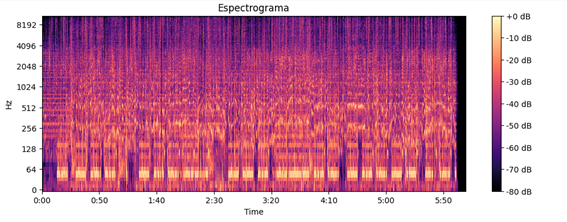
\includegraphics[width=.7\linewidth]{./Images/DatosExperimentales_2.png}
		\caption{}
	\end{center}
\end{figure}

\begin{figure}[H]
	\begin{center}
		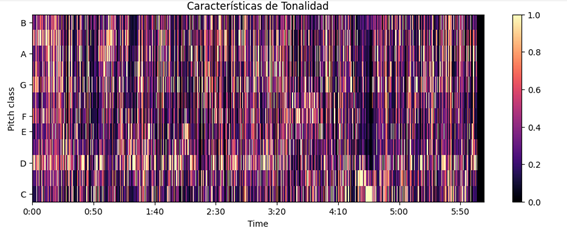
\includegraphics[width=.7\linewidth]{./Images/DatosExperimentales_3.png}
		\caption{}
	\end{center}
\end{figure}

\begin{figure}[H]
	\begin{center}
		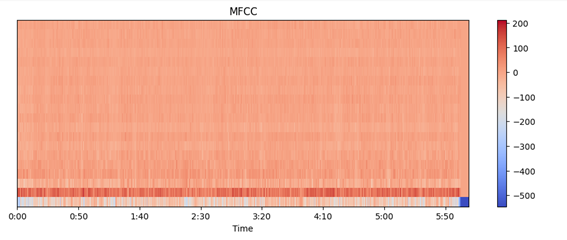
\includegraphics[width=.7\linewidth]{./Images/DatosExperimentales_4.png}
		\caption{}
	\end{center}
\end{figure}

% ! --------------------------------------------------------------------------------------------------------------------------------|>
\section*{Conclusiones}

En resumen, nuestro proyecto ``Lectura de Ondas'' ha
alcanzado logros significativos desarrollando un programa
capaz de leer y representar de manera óptima el
espectrograma y las propiedades fundamentales de las ondas
sonoras y a la vez abordamos uno de los desafíos
fundamentales: el filtrado de ondas sonoras para extraer
datos relevantes, lo que facilita el análisis preciso de
estas ondas. Estos avances establecen las bases de nuestro
proyecto y nos permite desarrollar y perfeccionar este.

\nocite{source_code}

\printbibliography

\end{document}